\subsection{Magacin}

\begin{figure}[ht]
\centering
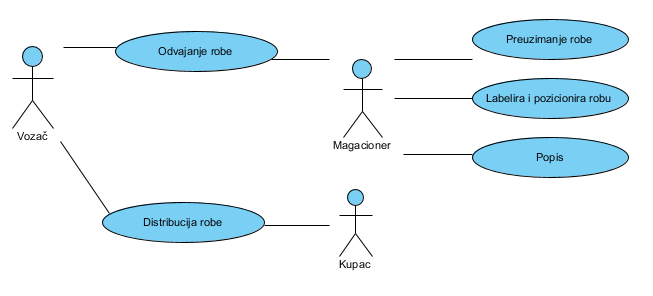
\includegraphics[width=140mm]{slike/useCaseMagacin.png}
\caption{Dijagram slučajeva upotrebe vezanih za magacin}
\end{figure}

\subsubsection{Prezimanje robe}

\textbf{Opis:}

Magacioner preuzima pristiglu robu od dostavljača zajedno sa prijemnicom.
\newline
\textbf{Akteri:}

Magacioner - preuzima robu i pregleda je
\newline
\textbf{Preduslov:}

Naručili smo robu od dobavljača.
\newline
\textbf{Postuslov:}

Roba je preuzeta i pozicionirana u magacinu.
\newline
\textbf{Glavni tok:}

1. Magacioner dočekuje robu od dobavljača i preuzima istu.

2. Kontroliše da li je sve u redu sa robom.

3. Pozicionira u magacinu pridošlu robu.
\newline
\textbf{Napomena:}

Prijemnicu takođe prima magacioner, pomoću nje kontroliše stanje i količinu robe.

\clearpage

\subsubsection{Labelira i pozicionira robu}

\textbf{Opis:}

Magacioner vodi evidenciju o organizaciji magacina. Gde se koji proizvodi nalaze i adekvatno ih obeležava. To unosi u program radi kasnijeg lakšeg snalaženja u pretrazi.
\newline
\textbf{Akteri:}

Magacioner - organizuje robu u magacinu
\newline
\textbf{Preduslov:}

Ima robe u magacinu.
\newline
\textbf{Postuslov:}

Roba je organizovana.
\newline
\textbf{Glavni tok:}

1. Magacioner pravi organizaciju raspoređivanja robe u magacinu.

2. Labelira robu.

3. Ulazi u deo programa prikaz magacina.

4. Unosi gde mu stoji koja roba.
\newline
\textbf{Napomena:}

Program ima jednostava grafički prikaz magacina, koji omogućava lakšu pretragu mogacionerima.

\subsubsection{Popis}

\textbf{Opis:}

Magacioner vrši popis stanja u magacinu, moguće je da se razlikuje od stanja magacina u programu. Možda je došlo do loma preparata ili je istekao rok ili se serije preparata ne poklapaju. Takođe slučajevi su i da nismo isporučili kupcu par komada lekova i on se nije bunio, ili je nama dobavljač greškom doneo više ili manje lekova.
\newline
\textbf{Akteri:}

Magacioner - vrši popis
\newline
\textbf{Preduslov:}

Ima robe u magacinu.
\newline
\textbf{Postuslov:}

Dobijeno realno stanje magacina.
\newline
\textbf{Glavni tok:}

1. Magacioner redom popisuje vrste lekova, seriju, količinu.

2. Dokument popis unosi u program, kome kasnije pristupa knjigovođa.

\clearpage

\subsubsection{Odvajanje robe}

\textbf{Opis:}

Magacioner po pristigloj otpremnici odvaja robu koja treba da se dostavi kupcu.
\newline
\textbf{Akteri:}

Magacioner - odvaja robu po otpremnici
\newline
\textbf{Preduslov:}

Otpremnica u magacinu.
\newline
\textbf{Postuslov:}

Roba je odvojena za transport.
\newline
\textbf{Glavni tok:}

1. Magacioner ulazi u deo programa za magacin, podsekcija otpremnice.

2. Obavlja odvajanje robe sa otpremnice.
\newline
\textbf{alternativni tok:}

2. U slučaju da nema odgovarajuće robe za odvajanje, javlja to komercijalisti, da se izradi nova adekvatna otpremnica.

\subsubsection{Distribucija robe}

\textbf{Opis:}

Magacioner zajedno sa vozačem utovaruje odvojenu robu,koju vozač dalje transportuje.
\newline
\textbf{Akteri:}

Magacioner - utovaruje robu

Vozač - utovaruje i transportuje robu
\newline
\textbf{Preduslov:}

Odvojena je roba po otpremnici.
\newline
\textbf{Postuslov:}

Roba je dostavljena kupcu.
\newline
\textbf{Glavni tok:}

1. Magacioner i vozač utovaruju robu u kamion.

2. Vozač dostavlja kupcu, robu i otpremnicu .

\clearpage